\documentclass{article}
\usepackage[utf8]{inputenc}
\usepackage[english,serbian]{babel}
\usepackage{amsmath}
\usepackage{enumitem}
\usepackage{graphicx}
\usepackage{float}
\usepackage{siunitx}
\usepackage[a4paper,left=1in,top=1in,right=1in,bottom=1in,nohead]{geometry}
\setlist[enumerate,1]{% (
leftmargin=*, itemsep=12pt, label={\textbf{\arabic*.}}}

\title{Prvi domaći zadatak iz Osnova elektronike}
\author{Luka Simić, 19/0368}
\date{}

\begin{document}

\begin{titlepage}
    \maketitle
\end{titlepage}

\section{Postavka}
\begin{enumerate}[itemsep=\baselineskip]
    \item Na slici \ref{KoloZadatak}, levo od tačaka $A$ i $B$ dato je glavno kolo sa strujno kontrolisanim strujnim generatorom čije je pojačanje Gain = 9. Desno od glavnog kola povezan je potrošač $R_p$ i kolo za merenje snage koje se sastoji od šanta $R_s=1m\Omega$ i idealnog množača (bibliotečka komponenta \textbf{mult}) koji generiše izlazni potencijal jednak proizvodu ulaznih potencijala. Šant je povezan redno sa potrošačem i dovoljno je mali ($R_p >> R_s$) da zanemarljivo utiče na rad celog kola, tako da je potencijal u tački $A$ praktično jednak padu napona na potrošaču. Pad napona na $R_s$ je proporcionalan struji kroz potrošač, što čini da je proizvod potencijala u tački $A$ i potencijala u tački $C$ proporcionalan snazi koja se dispira na potrošaču.
    \begin{figure}[H]
        \centering
        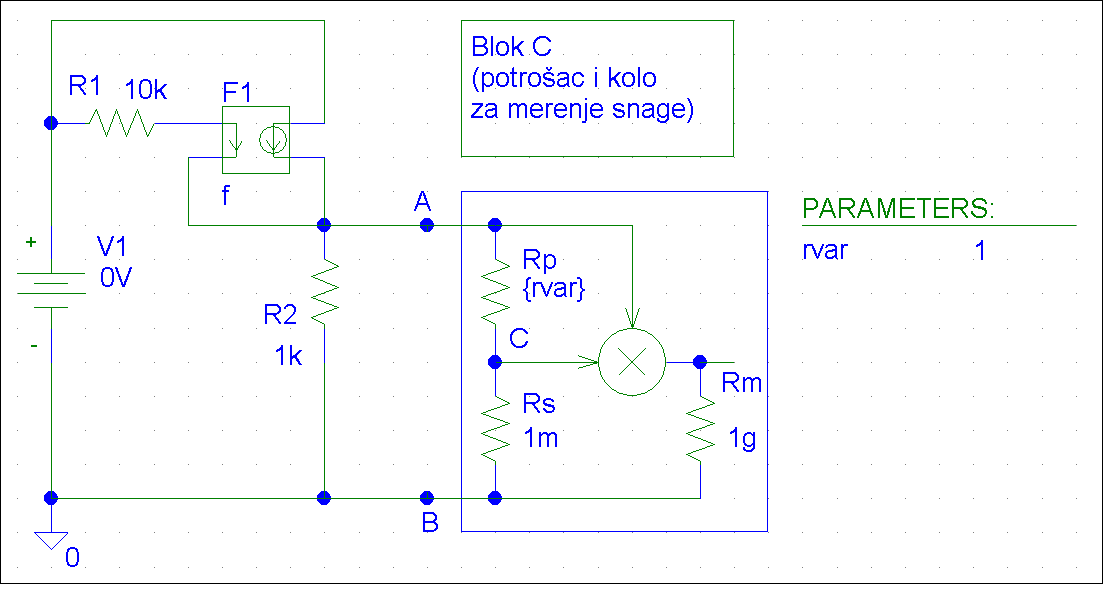
\includegraphics[width=275px]{Zadatak.png}
        \caption{Kolo sa strujno kontrolisanim strujnim generatorom F1}
        \label{KoloZadatak}
    \end{figure}
    \textbf{a)} [20] Ako se Blok $C$ (desno od tačaka $A$ i $B$) ukloni iz kola, računski odrediti ekvivalentni Tevenenov generator koji se vidi levo od tačaka $A$ i $B$.

    \textbf{b)} [20] Verifikovati rezultat dobijen u prethodnoj tački PSpice simulacijom.

    \textbf{c)} [20] Ako se između tačaka $A$ i $B$ poveže potrošač $R_{p_1}$, pri uklonjenom kompletnom Bloku $C$, izvesti računski vrednost potrošača $R_{p_1}$ na kome bi se razvila maksimalna moguća snaga.

    \textbf{d)} [40] Ako se posmatra kompletno kolo sa Slike 1, bez dodavanja ili oduzimanja bilo čega, korišćenjem DC Sweep analize globalnog parametra $rvar$, simulacijom i razmatranjem grafika snage odrediti vrednost potrošača $R_p$ na kome se razvija maksimalna moguća snaga.
\end{enumerate}

\section{Rešenje}
    \textbf{a)} Može se primetiti da će potencijal tačke $B$ kao i potencijal na negativnom kraju izvora napona biti isti kao potencijal uzemljenja, odnosno 0.
    \begin{equation}
        \label{GND}
        V_B = V_{gnd} = 0
    \end{equation}
    Odatle takođe vidimo kako je potencijal sa druge strane izvora napona jednak samom naponu $V_1$, i da će potencijal tačke $A$ biti jednak razlici napona $V_1$ i pada napona na otporniku $R_1$ ukoliko kroz njega prolazi struja $i_1$
    \begin{equation}
        \label{V1VA}
        V_A = V_1 - R_1 \times i_1
    \end{equation}
    S druge strane, vidimo da je potencijal tačke $B$ jednak razlici potencijala tačke $A$ i pada napona na otporniku $R_2$ ukoliko kroz njega prolazi struja $i_2$.
    \begin{equation}
        \label{VAVB}
        V_A - i_2 \times R_2 = V_B
    \end{equation}
    U čvoru $A$ sreću se tri struje, $i_1$, $i_2$ kao i devetostruka vrednost $i_1$ koju generiše zavisni strujni generator, tako da iz Kirhofovog zakona za struje zaključujemo:
    \begin{equation}
        \label{I}
        i_2 = i_1 + 9i_1 = 10i_1
    \end{equation}
    Kombinacijom \eqref{GND}, \eqref{V1VA}, \eqref{VAVB} i \eqref{I} dobijamo jednačine:
    $$V_1 - R_1 \times i_1 - 10i_1 \times R_2 = 0$$
    $$V_1 = i_1 \times (R_1 + 10R_2)$$
    \begin{equation}
        \label{Combined 1}
        i_1 = \frac{V_1}{R_1 + 10R_2}
    \end{equation}
    Pa tako iz \eqref{V1VA} i \eqref{Combined 1} dobijamo da je:
    $$V_A = V_1 - R_1 \times \frac{V_1}{R_1 + 10R_2}$$
    $$V_A = V_1 \times \frac{R_1 + 10R_2 - R_1}{R_1 + 10R_2}$$
    \begin{equation}
        \label{Combined 2}
        V_A = V_1 \times \frac{10R_2}{R_1 + 10R_2}
    \end{equation}
    Ubacivanjem vrednosti u \eqref{Combined 2} dobijamo:
    $$V_A = V_1 \times \frac{10 \times 1k\Omega}{10k\Omega + 10 \times 1k\Omega}$$
    $$V_A = V_1 \times \frac{10k\Omega}{20k\Omega}$$
    $$V_A = \frac{V_1}{2}$$
    Pošto je napon u tački $B$ jednak nuli, time dobijamo da je ovo konačno rešenje.
    $$U_t = \frac{V_1}{2}$$

    Za određivanje ekvivalentnog otpora između tačaka $A$ i $B$ prvo zamenjujemo nezavisni naponski generator s naponom $V_1$ kratkim spojem a zatim povezujemo test generator napona $v_t$ između čvorova $A$ i $B$ i smatramo da kroz tu granu prolazi struja $i_t$ u smeru od $B$ ka $A$. Iz Kirhofovog zakona za struje za čvor A sada dobijamo:
    \begin{equation}
        \label{I2}
        i_{R_2} = i_1 + 9i_1 + i_t = 10i_1 + i_t
    \end{equation}
    Pošto je test generator jedini generator napona povezan između čvorova $A$ i $B$, iz \eqref{GND} dobijamo da je potencijal tačke $A$ jednak naponu koji generiše test generator.
    \begin{equation}
        \label{VAvt}
        v_t = V_A - V_B = V_A
    \end{equation}
    Sa izbačenim nezavisnim generatorom napona sada imamo ukupno dva čvora u kolu i između njih su povezani otpornici od $1k\Omega$ i $10k\Omega$ tako da, slično kao u \eqref{V1VA} i \eqref{VAVB} dobijamo:
    \begin{equation}
        \label{VAVB2}
        V_A = V_B - i_1 \times R_1
    \end{equation}
    \begin{equation}
        \label{VAVB3}
        V_B = V_A - i_{R_2} \times R_2
    \end{equation}
    Kombinacijom \eqref{VAVB2}, \eqref{VAVB3}, \eqref{I2} i \eqref{GND} dobijamo:
    $$0 = 0 - i_1 \times R_1 - (10i_1 + i_t) \times R_2$$
    $$i_1 \times (R_1 + 10R_2) = -i_t \times R_2$$
    \begin{equation}
        \label{it}
        i_t = -i_1\frac{R_1 + 10R_2}{R_2}
    \end{equation}
    A kombinacijom \eqref{VAVB2}, \eqref{VAvt} i \eqref{GND} dobijamo:
    \begin{equation}
        \label{vti1}
        v_t = -i_1 \times R_1
    \end{equation}
    Otpor ekvivalentnog Tevenenovog generatora je određen jednačinom:
    \begin{equation}
        \label{Rt}
        R_t = \frac{v_t}{i_t}
    \end{equation}
    Pa iz \eqref{Rt}, \eqref{VAvt} i \eqref{vti1} dobijamo:
    $$R_t = \frac{-i_1 \times R_1}{-i_1\frac{R_1 + 10R_2}{R_2}}$$
    \begin{equation}
        \label{Rt2}
        R_t = \frac{R_1}{\frac{R_1 + 10R_2}{R_2}}
    \end{equation}
    Ubacivanjem vrednosti $R_1$ i $R_2$ u \eqref{Rt2} dobijamo konačno rešenje:
    $$R_t = \frac{10k\Omega}{\frac{10k\Omega + 10 \times 1k\Omega}{1k\Omega}}$$
    $$R_t = \frac{10k\Omega}{20}$$
    $$R_t = \frac{1}{2}k\Omega = 500\Omega$$

    \textbf{b)} Kola pomenuta u prvom delu zadatka se mogu videti na slikama \ref{KoloUt} i \ref{KoloRt}.

    U slučaju verifikacije napona, napon na $V_1$ postavljen je na vrednost od 5V. Nakon simulacije, PSpice je pokazivao potencijal od 2.5V u tački $A$ i 0V u tački B, što pokazuje da je napon između ove dve tačke zaista polovina od $V_1$ kao što je izračunato u računskom delu zadatka.
    \begin{figure}[H]
        \centering
        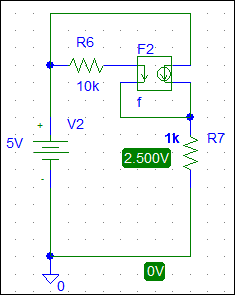
\includegraphics[width=120px]{KoloZaVerifikacijuTevenenovogNapona.png}
        \caption{Kolo za verifikaciju Tevenenovog napona}
        \label{KoloUt}
    \end{figure}

    U slučaju verifikacije otpora, napon test generatora je postavljen na 5V. Nakon simulacije, PSpice je pokazivao struju od 10mA kroz granu sa test generatorom, što pokazuje da je ekvivalentni otpor Tevenenovog generatora koji se računa kao količnik ove dve vrednosti zaista $500\Omega$ kao što je izračunato u računskom delu zadatka.
    \begin{figure}[H]
        \centering
        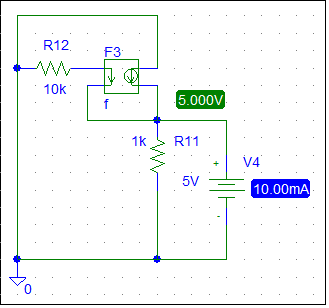
\includegraphics[width=180px]{KoloZaVerifikacijuTevenenovogOtpora.png}
        \caption{Kolo za verifikaciju Tevenenovog otpora}
        \label{KoloRt}
    \end{figure}

    \textbf{c)} Ukoliko ekvivalentiramo kolo levo od tačaka $A$ i $B$ Tevenenovim generatorom čije smo parametre izračunali u prvom delu zadatka, dobijamo kolo sa redno vezanim generatorom napona jačine $\frac{V_1}{2}$ i dva otpornika otpornosti $500\Omega$ i $R_{p_1}$. Jednačina snage koja se disipira na otporniku jeste:
    \begin{equation}
        \label{P}
        P = I^2 \times R
    \end{equation}
    Ekvivalentni otpor u ovom kolu možemo izračunati kao zbir otpornosti dva redno vezana otpornika, i na taj način odrediti struju koja kroz njih prolazi.
    \begin{equation}
        \label{I3}
        I = \frac{\frac{V1}{2}}{500\Omega + R_{p_1}}
    \end{equation}
    Iz \eqref{P} i \eqref{I3} možemo izraziti snagu koja prolazi kroz otpornik otpornosti $R_{p_1}$ kao funkciju u zavisnosti od $R_{p_1}$:
    \begin{equation}
        \label{PRp1}
        P_{R_{p_1}}(R_{p_1}) = (\frac{\frac{V1}{2}}{500\Omega + R_{p_1}})^2 \times R_{p_1}
    \end{equation}
    Kada je izvod funkcije \eqref{PRp1} jednak nuli dobijamo da je snaga najveća, tako da iz te jednačine možemo pronaći vrednost otpora $R_{p_1}$ za najveću snagu. Ukoliko pretpostavimo da napon $V_1$ nije nula:
    $$\frac{\partial P_{R_{p_1}}}{\partial R_{p_1}} = 0$$
    $$-\frac{(R_{p_1} - 500\Omega) \times V_1^2}{4 (R_{p_1} + 500\Omega)^3} = 0$$
    $$R_{p_1} = 500\Omega$$

    \textbf{d)} Nakon sastavljanja traženog kola kao na slici \ref{KoloP}, sa dobijenog grafika (slika \ref{Grafik}) se može videti da je snaga maksimalna za $R_p = 500\Omega$. Ovaj rezultat je isti kao rezultat iz trećeg dela zadatka jer je struja kroz otpornik $R_m$ zanemarljiva (otpornik ima veoma veliku otpornost), pad napona na otporniku $R_s$ je isto zanemarljiv (otpornik ima veoma malu otpornost) a kroz idealni množač ne teče struja (množač je varijanta operacionog pojačavača).

    \begin{figure}[H]
        \centering
        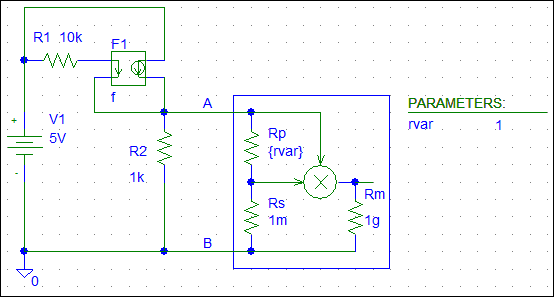
\includegraphics[width=275px]{KoloP.png}
        \caption{Kolo za merenje snage na potrošaču $R_p$}
        \label{KoloP}
    \end{figure}

    \begin{figure}[H]
        \centering
        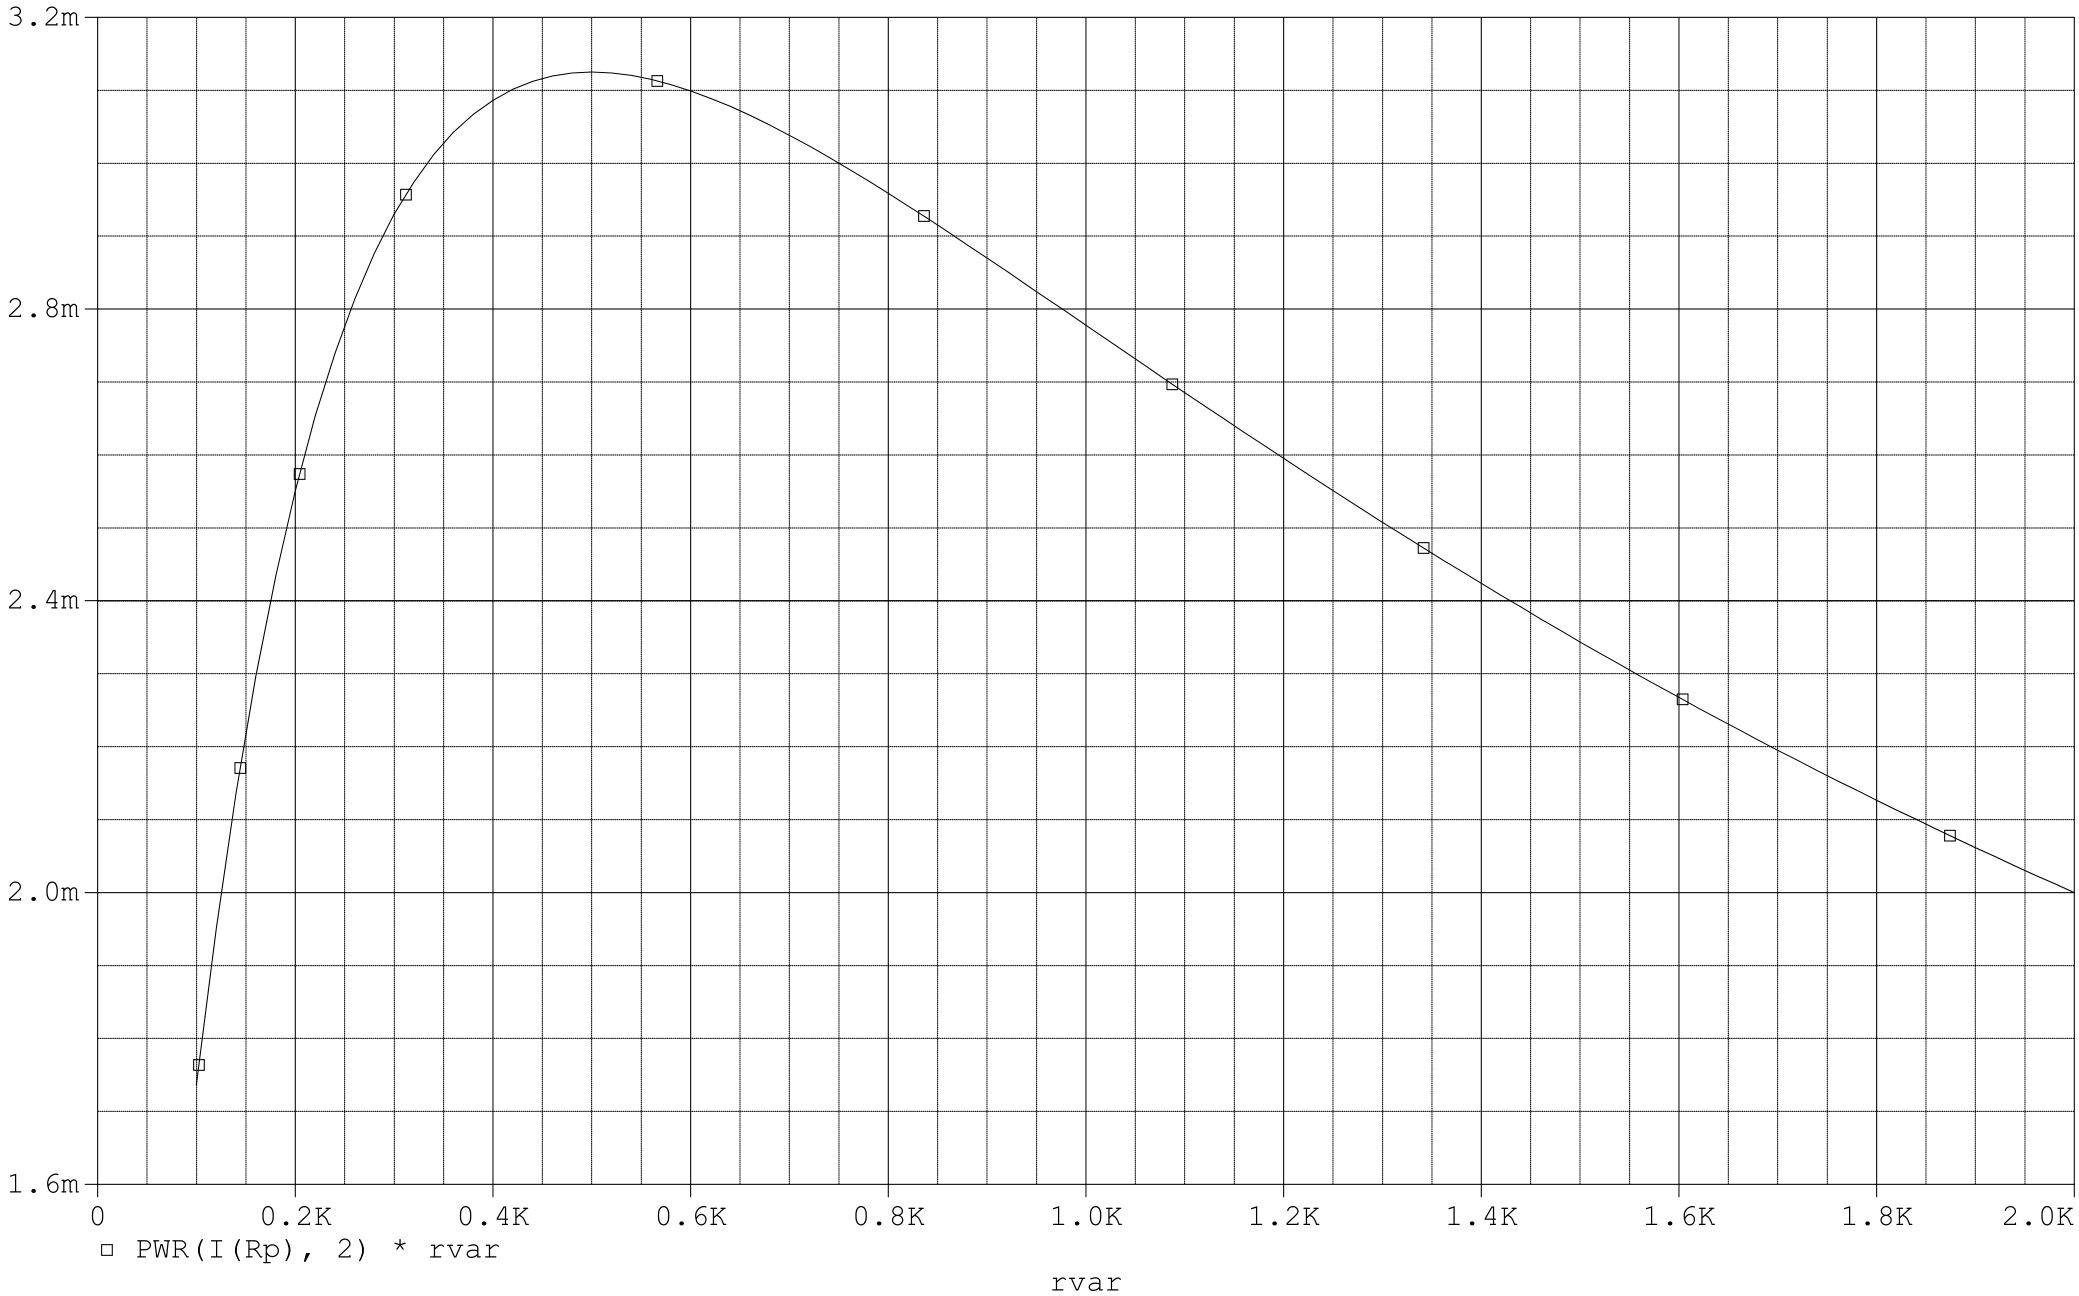
\includegraphics[width=400px]{Grafik.png}
        \caption{Dobijeni grafik zavisnosti snage na potrošaču $R_p$ od otpornosti}
        \label{Grafik}
    \end{figure}

\end{document}
